\section{Precision of system}\label{sec:precisionofsystem}

This experiment will test the precision of the complete system with the parameters found in \ref{section:}

\subsection{Range}

The system will change between two different positions, and stop when it has reached as it best can. When controller stops the position are marked, and the other position is set to the controller which now converges to this position. When it reaches it the position are marked and it will begin moving to the former position etc. \dots This is done ten times.

\subsection{Test Setup}\label{subsec:testsetup}

The test is performed by fastening a laser pointer on the pan/tilt system. A board is placed next to the system and two positions were the pointer is on the board are chosen \ref{fig:systemtestsetup}. The laser pointer is placed 174 cm and 180.5 from each point. Thus each degree is at around 3 centimetres wide.

\[ \frac{\Pi*2*174}{360} = 3.03687 \]


\begin{figure}[htb]
	\centering
	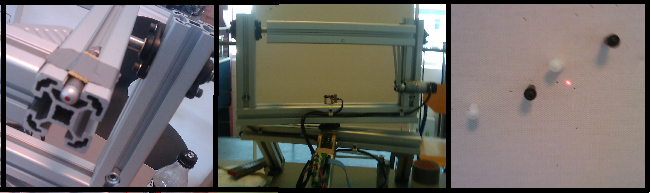
\includegraphics[width=\textwidth,trim=0 0 0 0]{graphics/overallsystemtest.png} %trim=l b r t (can cut off from every side)
	\caption{Setup if the test. From left to right; the mounted laser, the system pointing at the board, laser dot and marks.}
	\label{fig:systemtestsetup}			% figure labels are of the form \label{fig:*}
\end{figure}


\subsection{Result}

At both points the error was less than five centimetres and at most of the time less than two. This means that the system have an uncertainty between 0.658 and 3.293 degrees. This precision is reached with overshoot.

\[ \frac{2.0}{3.03687} = 0.658 \]

\[ \frac{10.0}{3.03687} = 3.293 \]

\subsection{Conclusion}

The system itself, have a precision of af third degree.
\[ \frac{360}{160} = 1/3 \]

It is a high precision that have been observed, at times the uncertainty is as small as the precision of the system. Though it does also show that a higher precision can be obtained. Overshooting was though occurring in the control.

\section{Precision of new parameters}\label{sec:precisionofsystem2}

This experiment will test the PID values found at \ref{sec:}

\subsection{Range}

Here the system will change between two position but only one of the positions are marked. This is repeated ten times.

\subsection{Test Setup}

The setup will be the same as the above \ref{sec:precisionofsystem}, see Figure \ref{fig:systemtestsetup}, with the exception that only one point is measured at the distance 370 centimetres. Thus each degree is 6.458 centimetres wide.

\[ \frac{\Pi*2*370}{360} = 6.458 \]

\subsection{Result}

In this test the precision of the pan and tilt were recorded to be quite different. For the tilt was the points precision 7 centimetres were all the points at the tilt was inside two centimetres. Thus the pan/tilt system have reached precision of respectively 0.310 degrees and 1.083 degrees.


\[ \frac{2}{6.458} = 0.310 \]

\[ \frac{7}{6.458} = 1.083 \]

\subsection{Conclusion}

Thus the pan have reached a constant precision on par with the systems precision of a third. The tilt part have also become more precise, but it should be possible to make it more precise. It could be that because the tilt is affected by gravity it is harder to control and thus the harder to control.  The system is though not able to hit the position without overshooting. But as precision and not speed was our objective this is a very satisfying result.